\documentclass{book}
\usepackage{commeunjeustyle}

\begin{document}

\chapter*{Structures algébriques}
\begin{Texte}
L'enfant, après avoir appris 
\begin{itemize}
\item à \impo{compter} le nombre d'objets en ajoutant des unités à partir de 0 c'est à dire en construisant l'ensemble $\N$  avec l'opération "suivant"
\begin{center}
\begin{tikzpicture}
\draw[color=colorprop] (0,0) rectangle (1,1);
\node at (0.5,-0.3){$0$};
\draw[color=colorprop] (1.5,0) rectangle (2.5,1);
\draw[color=colordef] (2,0.5) circle (0.15);
\node at (2,-0.3){$1$};
\draw[color=colorprop] (3,0) rectangle (4,1);
\draw[color=colordef] (3.3,0.2) circle (0.15);
\draw[color=colordef] (3.7,0.7) circle (0.15);
\node at (3.5,-0.3){$2$};
\draw[color=colorprop] (4.5,0) rectangle (5.5,1);
\draw[color=colordef] (4.8,0.75) circle (0.15);
\draw[color=colordef] (4.7,0.2) circle (0.15);
\draw[color=colordef] (5.3,0.5) circle (0.15);
\node at (5,-0.3){$3$};
\end{tikzpicture}\\
Désignation à l'aide d'un nombre de la quantité de cercles 
\end{center}
\item à \impo{ordonner} en comparant des quantités c'est à munir d'une structure d'ordre à l'ensemble $\N$ 
\begin{center}
\begin{tikzpicture}
\draw[color=colorprop] (1.5,0) rectangle (2.5,1);
\draw[color=colordef] (2,0.5) circle (0.15);
\node at (3,0.5){$\leq$};
\draw[color=colorprop] (3.5,0) rectangle (4.5,1);
\draw[color=colordef] (3.8,0.75) circle (0.15);
\draw[color=colordef] (3.7,0.2) circle (0.15);
\draw[color=colordef] (4.3,0.5) circle (0.15);
\end{tikzpicture}\\
Comparaison de deux quantités de cercles 
\end{center}
\end{itemize}
commence
\begin{itemize}
\item  à \impo{additionner} les nombres en opérant des regroupements.
\begin{center}
\begin{tikzpicture}
\draw[color=colorprop,fill=colorprop!20] (0,0) rectangle (1,1);
\draw[color=colorprop,fill=colorprop!20] (1,0) rectangle (2,1);
\draw[color=colorprop,fill=colorprop!20] (2,0) rectangle (3,1);
\node at (1,-0.5){$3$};
\node at (3.5,0.5){$+$};
\node at (3.5,-0.5){$+$};
\draw[color=colordef,fill=colordef!20] (4,0) rectangle (5,1);
\draw[color=colordef,fill=colordef!20] (5,0) rectangle (6,1);
\node at (5,-0.5){$2$};
\node at (6.5,0.5){$=$};
\node at (6.5,-0.5){$=$};
\draw[color=colorprop,fill=colorprop!20] (7,0) rectangle (8,1);
\draw[color=colorprop,fill=colorprop!20] (8,0) rectangle (9,1);
\draw[color=colorprop,fill=colorprop!20] (9,0) rectangle (10,1);
\draw[color=colordef,fill=colordef!20] (10,0) rectangle (11,1);
\draw[color=colordef,fill=colordef!20] (11,0) rectangle (12,1);
\node at (9.5,-0.5){$5$};
\end{tikzpicture}\\
Regroupement de cubes pour additionner
\end{center}
\item  à \impo{multiplier} les nombres en opérant une addition itérée.
\begin{center}
\begin{tikzpicture}
\draw[color=colorprop,fill=colorprop!20] (-10,0) rectangle (-9,1);
\draw[color=colorprop,fill=colorprop!20] (-10,1) rectangle (-9,2);
\node[scale=2] at (-8.5,1){$+$};
\draw[color=colorprop,fill=colorprop!20] (-8,0) rectangle (-7,1);
\draw[color=colorprop,fill=colorprop!20] (-8,1) rectangle (-7,2);
\node[scale=2] at (-6.5,1){$+$};
\draw[color=colorprop,fill=colorprop!20] (-6,0) rectangle (-5,1);
\draw[color=colorprop,fill=colorprop!20] (-6,1) rectangle (-5,2);
\node[scale=2] at (-4.5,1){$=$};
\draw[color=colorprop,fill=colorprop!20] (-4,0) rectangle (-3,1);
\draw[color=colorprop,fill=colorprop!20] (-3,0) rectangle (-2,1);
\draw[color=colorprop,fill=colorprop!20] (-2,0) rectangle (-1,1);
\draw[color=colorprop,fill=colorprop!20] (-4,1) rectangle (-3,2);
\draw[color=colorprop,fill=colorprop!20] (-3,1) rectangle (-2,2);
\draw[color=colorprop,fill=colorprop!20] (-2,1) rectangle (-1,2);
\node at (-5,-0.5) {$\overbrace{2+2+2}^{3 \text{ fois}}\quad=\quad 3\times 2$};
\end{tikzpicture}\\
Regroupement itéré de cubes pour multiplier
\end{center}
 \end{itemize}
puis s'intéresse aux propriétés des opérations :
\begin{itemize}
 \item \impo{associativité} de l'addition $(a+b)+c=a+(b+c)$ et de la multiplication $(a\times b)\times c=a\times(b \times c)$
\begin{center}
\begin{tikzpicture}[scale=0.75]
\node[scale=2] at (-0.2,0.5){$($};
\draw[color=colorprop,fill=colorprop!20] (0,0) rectangle (1,1);
\draw[color=colorprop,fill=colorprop!20] (1,0) rectangle (2,1);
\draw[color=colorprop,fill=colorprop!20] (2,0) rectangle (3,1);
\node[scale=2] at (3.5,0.5){$+$};
\draw[color=colordef,fill=colordef!20] (4,0) rectangle (5,1);
\draw[color=colordef,fill=colordef!20] (5,0) rectangle (6,1);
\node[scale=2] at (6.5,0.5){$)+$};
\draw[color=green,fill=green!20] (7,0) rectangle (8,1);
\node[scale=2] at (8.5,0.5){$=$};
\draw[color=colorprop,fill=colorprop!20] (9,0) rectangle (10,1);
\draw[color=colorprop,fill=colorprop!20] (10,0) rectangle (11,1);
\draw[color=colorprop,fill=colorprop!20] (11,0) rectangle (12,1);
\draw[color=colordef,fill=colordef!20] (12,0) rectangle (13,1);
\draw[color=colordef,fill=colordef!20] (13,0) rectangle (14,1);
\node[scale=2] at (14.5,0.5){$+$};
\draw[color=green,fill=green!20] (15,0) rectangle (16,1);
\node[scale=2] at (16.5,0.5){$=$};
\draw[color=colorprop,fill=colorprop!20] (17,0) rectangle (18,1);
\draw[color=colorprop,fill=colorprop!20] (18,0) rectangle (19,1);
\draw[color=colorprop,fill=colorprop!20] (19,0) rectangle (20,1);
\draw[color=colordef,fill=colordef!20] (20,0) rectangle (21,1);
\draw[color=colordef,fill=colordef!20] (21,0) rectangle (22,1);
\draw[color=green,fill=green!20] (22,0) rectangle (23,1);


\draw[color=colorprop,fill=colorprop!20] (0,-1) rectangle (1,-2);
\draw[color=colorprop,fill=colorprop!20] (1,-1) rectangle (2,-2);
\draw[color=colorprop,fill=colorprop!20] (2,-1) rectangle (3,-2);
\draw[color=colordef,fill=colordef!20] (3,-1) rectangle (4,-2);
\draw[color=colordef,fill=colordef!20] (4,-1) rectangle (5,-2);
\draw[color=green,fill=green!20] (5,-1) rectangle (6,-2);
\node[scale=2] at (6.5,-1.5){$=$};
\draw[color=colorprop,fill=colorprop!20] (7,-1) rectangle (8,-2);
\draw[color=colorprop,fill=colorprop!20] (8,-1) rectangle (9,-2);
\draw[color=colorprop,fill=colorprop!20] (9,-1) rectangle (10,-2);
\node[scale=2] at (10.5,-1.5){$+$};
\draw[color=colordef,fill=colordef!20] (11,-1) rectangle (12,-2);
\draw[color=colordef,fill=colordef!20] (12,-1) rectangle (13,-2);
\draw[color=green,fill=green!20] (13,-1) rectangle (14,-2);
\node[scale=2] at (14.5,-1.5){$=$};
\draw[color=colorprop,fill=colorprop!20] (15,-1) rectangle (16,-2);
\draw[color=colorprop,fill=colorprop!20] (16,-1) rectangle (17,-2);
\draw[color=colorprop,fill=colorprop!20] (17,-1) rectangle (18,-2);
\node[scale=2] at (18.5,-1.5){$+($};
\draw[color=colordef,fill=colordef!20] (19,-1) rectangle (20,-2);
\draw[color=colordef,fill=colordef!20] (20,-1) rectangle (21,-2);
\node[scale=2] at (21.5,-1.5){$+$};
\draw[color=green,fill=green!20] (22,-1) rectangle (23,-2);
\node[scale=2] at (23.2,-1.5){$)$};
\end{tikzpicture}\\
Démonstration géométrique élémentaire de l'associativité  de l'addition
\end{center}
\item \impo{commutativité} de l'addition $a+b=b+a$ et de la multiplication $a\times b=b\times a$
\begin{center}
\begin{tikzpicture}
\draw[color=colorprop,fill=colorprop!20] (0,0) rectangle (1,1);
\draw[color=colorprop,fill=colorprop!20] (1,0) rectangle (2,1);
\draw[color=colorprop,fill=colorprop!20] (2,0) rectangle (3,1);
\draw[color=colordef,fill=colordef!20] (0,1) rectangle (1,2);
\draw[color=colordef,fill=colordef!20] (1,1) rectangle (2,2);
\draw[color=colordef,fill=colordef!20] (2,1) rectangle (3,2);
\node[scale=2] at (-0.5,1){$=$};
\draw[color=colorprop,fill=colorprop!20] (-4,0) rectangle (-3,1);
\draw[color=colordef,fill=colordef!20] (-3,0) rectangle (-2,1);
\draw[color=green,fill=green!20] (-2,0) rectangle (-1,1);
\draw[color=colorprop,fill=colorprop!20] (-4,1) rectangle (-3,2);
\draw[color=colordef,fill=colordef!20] (-3,1) rectangle (-2,2);
\draw[color=green,fill=green!20] (-2,1) rectangle (-1,2);
\node at (-1,-0.5) {$\overbrace{a}^{\text{Nombre de colonnes}}\times \overbrace{b}^{\text{Nombre de cubes par colonne}}\quad=\quad \overbrace{b}^{\text{Nombre de lignes}}\times \overbrace{a}^{\text{Nombre de cubes par ligne}}$};
\end{tikzpicture}\\
Démonstration géométrique élémentaire de la commutativité  de la multiplication
\end{center}
\item \impo{distributivité} de la multiplication sur l'addition $a\times (b+c)=(a\times b)+(a\times c) $
\begin{center}
\begin{tikzpicture}
\draw[color=colordef,fill=colordef!20] (-10,2) rectangle (-9,3);
\draw[color=colorprop,fill=colorprop!20] (-10,0) rectangle (-9,1);
\draw[color=colorprop,fill=colorprop!20] (-10,1) rectangle (-9,2);
\node[scale=2] at (-8.5,1.5){$+$};
\draw[color=colordef,fill=colordef!20] (-8,2) rectangle (-7,3);
\draw[color=colorprop,fill=colorprop!20] (-8,0) rectangle (-7,1);
\draw[color=colorprop,fill=colorprop!20] (-8,1) rectangle (-7,2);
\node[scale=2] at (-6.5,1.5){$+$};
\draw[color=colordef,fill=colordef!20] (-6,2) rectangle (-5,3);
\draw[color=colorprop,fill=colorprop!20] (-6,0) rectangle (-5,1);
\draw[color=colorprop,fill=colorprop!20] (-6,1) rectangle (-5,2);
\node[scale=2] at (-4.5,1.5){$=$};
\draw[color=colorprop,fill=colorprop!20] (-4,0) rectangle (-3,1);
\draw[color=colorprop,fill=colorprop!20] (-3,0) rectangle (-2,1);
\draw[color=colorprop,fill=colorprop!20] (-2,0) rectangle (-1,1);
\draw[color=colorprop,fill=colorprop!20] (-4,1) rectangle (-3,2);
\draw[color=colorprop,fill=colorprop!20] (-3,1) rectangle (-2,2);
\draw[color=colorprop,fill=colorprop!20] (-2,1) rectangle (-1,2);
\draw[color=colordef,fill=colordef!20] (-4,2) rectangle (-3,3);
\draw[color=colordef,fill=colordef!20] (-3,2) rectangle (-2,3);
\draw[color=colordef,fill=colordef!20] (-2,2) rectangle (-1,3);

\draw[color=colorprop,fill=colorprop!20] (-10,-4) rectangle (-9,-3);
\draw[color=colorprop,fill=colorprop!20] (-9,-4) rectangle (-8,-3);
\draw[color=colorprop,fill=colorprop!20] (-8,-4) rectangle (-7,-3);
\draw[color=colorprop,fill=colorprop!20] (-10,-3) rectangle (-9,-2);
\draw[color=colorprop,fill=colorprop!20] (-9,-3) rectangle (-8,-2);
\draw[color=colorprop,fill=colorprop!20] (-8,-3) rectangle (-7,-2);
\draw[color=colordef,fill=colordef!20] (-10,-2) rectangle (-9,-1);
\draw[color=colordef,fill=colordef!20] (-9,-2) rectangle (-8,-1);
\draw[color=colordef,fill=colordef!20] (-8,-2) rectangle (-7,-1);
\node[scale=2] at (-6.5,-2.5){$=$};
\draw[color=colorprop,fill=colorprop!20] (-6,-4.5) rectangle (-5,-3.5);
\draw[color=colorprop,fill=colorprop!20] (-5,-4.5) rectangle (-4,-3.5);
\draw[color=colorprop,fill=colorprop!20] (-4,-4.5) rectangle (-3,-3.5);
\draw[color=colorprop,fill=colorprop!20] (-6,-3.5) rectangle (-5,-2.5);
\draw[color=colorprop,fill=colorprop!20] (-5,-3.5) rectangle (-4,-2.5);
\draw[color=colorprop,fill=colorprop!20] (-4,-3.5) rectangle (-3,-2.5);
\node[scale=2] at (-4.5,-2){$+$};
\draw[color=colordef,fill=colordef!20] (-6,-1.5) rectangle (-5,-0.5);
\draw[color=colordef,fill=colordef!20] (-5,-1.5) rectangle (-4,-0.5);
\draw[color=colordef,fill=colordef!20] (-4,-1.5) rectangle (-3,-0.5);

\end{tikzpicture}\\
Démonstration géométrique élémentaire de la distributivité  $\overbrace{(b+c)+\dots+(b+c)}^{a \text{ fois}}\quad=\quad  ( \overbrace{b+\dots+b}^{a \text{ fois}})+(\overbrace{c+\dots+c}^{a \text{ fois}})$
\end{center}
 \end{itemize}
ensuite après avoir défini $0$ comme l'\impo{élément neutre} de l'addition (additionner $0$ à un nombre donne ce même nombre) 
\begin{center}
 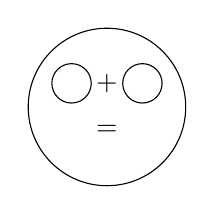
\begin{tikzpicture}
\draw (0,0) circle (1);
\draw (-0.45,0.3) circle (0.25);
\node at (0,0.3){$+$};
\draw (+0.45,0.3) circle (0.25);
\node at (0,-0.3){$=$};
\end{tikzpicture}\\
Cas particulier bien connu 0+0=0
\end{center}
  on construit l'ensemble des entiers relatifs à partir de l'\impo{opposé} d'un entier naturel :
$$\begin{aligned}
2+(2-4)&=&(2+2)-4&=&0\\
2+(1-3)&=&(2+1)-3&=&0\\
2+(0-2)&=&(2+0)-2&=&0\\
\end{aligned}$$
Ainsi "en supprimant le zéro", 
$$2+(-2)=0.$$
le nombre négatif $-2$ "naît".\\ 
Dans le supérieur, nous rencontrons de nombreux ensembles : les entiers naturels, les entiers relatifs, les fractions, les réels, les complexes, les polynômes, les vecteurs, les matrices, les fonctions continues etc. L'objectif de ce cours est de suivre le cheminement de l'enfant en généralisant à un ensemble  $A$  quelconque et non plus l'ensemble des entiers.\\
Structurer un ensemble $A$ avec une relation d'ordre $\leq$ pour définir un ensemble ordonné $(A\leq)$ sera faite dans un autre cours.  Comme un enfant aimant additionner et multiplier, un Mathématicien souhaite structurer un ensemble avec des opérations appelées \impo{lois de composition} qu'il appelle une \impo{structure algébrique}. L'addition et la multiplication  obéissent à plusieurs propriétés algébriques : l'associativité et la commutativité. De nombreuses structures algébriques étudiées obéissent à certaines, mais pas nécessairement à toutes, de ces lois. \\
$0$ est un élément particulier de l'addition appelé l'\impo{élément neutre} c'est à dire il laissent tous les autres éléments inchangés lorsqu'il est composé avec eux. On se posera la question d'existence et d'unicité de l'élément neutre. La notion d'\impo{élément symétrique} généralise le concept d'opposé en rapport avec l'addition.\\
%l'element neutre est central : résolutuon d'équation et construction de Z et Q 
Enfin, on étudiera une première structure algébrique appelé \impo{groupe}.    
\end{Texte}


%%%%%%%%%%%%%%%%%%%%%%%%%%%%%%%%%%%%%%%%%%%%%%%%%%%%%%%%%%%%%%%%%%%%%%
\section{Loi de composition}
\subsection{Définition}
\begin{Definition}[Loi de composition interne]
Soit $A$ un ensemble.\\
Une \defi{loi de composition interne}, $\bigtriangleup$, est une application qui, à deux éléments de $A$, associe un élément de $A$ :
$$ \Fonction{\bigtriangleup}{A\times A}{A}{(x,y)}{x \bigtriangleup y}.$$
\end{Definition}
\begin{Exemple}
\begin{itemize}
\item Sur $\R$, l'addition définie par $\Fonction{+}{\R\times \R}{\R}{(x,y)}{x + y}$, la soustraction $\Fonction{-}{\R\times \R}{\R}{(x,y)}{x - y}$ et la multiplication $\Fonction{-}{\R\times \R}{\R}{(x,y)}{x \times y}$ sont des lois de composition internes.
\item Sur $\N$, la soustraction n'est pas une loi interne, mais elle l'est dans $\Z$.
\item Sur $\N^*$,  l'exponentiation définie par $\Fonction{}{\N^*\times\N^*}{\N^*}{(a,b)}{a^b}$, le PGCD ou le PPCM sont des lois internes.
\item Soit $X$ un ensemble. Sur l'ensemble des parties de $X$, $\mathcal{P}(X)$, l'union définie par $\Fonction{\cup}{\mathcal{P}(X)\times \mathcal{P}(X)}{\mathcal{P}(X)}{(A,B)}{A \cup B}$ et l'intersection $\Fonction{\cap}{\mathcal{P}(X)\times \mathcal{P}(X)}{\mathcal{P}(X)}{(A,B)}{A \cap B}$ sont des lois de composition internes.
\end{itemize}
\end{Exemple}

\begin{Definition}[Loi de composition externe] 
Soit $X$ et $A$ deux ensembles.\\
Une \defi{loi de composition externe}, $.$, est une application qui, à un élément de $X$ et un élément de $A$, associe un élément de $A$ :
$$ \Fonction{.}{X\times A}{A}{(\lambda,x)}{\lambda. x} $$
\end{Definition}
\begin{Exemple}[\((\R^2,.)\)]
La multiplication par un scalaire sur l'ensemble des vecteurs du plan  $\R^2$ définie par 
$$ \Fonction{.}{\R\times\R^2}{\R^2}{(\lambda,(x_1,x_2))}{(\lambda.x_1, \lambda.x_2)}.$$ est une loi de composition externe.
\end{Exemple}


\subsection{Propriétés éventuelles des lois de composition interne}
\begin{Definition}[Commutativité et associativité]
$\bigtriangleup$ est
\begin{enumerate}
\item  \defi{associative} : si $\in(x,y,z)\in A^3$, $x \bigtriangleup (y \bigtriangleup z) = (x \bigtriangleup y) \bigtriangleup z$.
  On ne considèrera que des loi associatives.
\item
 \defi{commutative} : si $\forall(x,y)\in A^2$, $x \bigtriangleup y = y \bigtriangleup x$.
 \end{enumerate}
\end{Definition} 
 \begin{Exemple}
\begin{itemize}
\item Sur $\R$, l'addition et la multiplication sont commutatives et associatives. Ce n'est pas le cas de la soustraction car $1-0\neq 0-1$ et $1-(2-3)=2\neq -4= (1-2)-3.$
\item Sur $\N^*$,  l'exponentiation n'est pas commutative $1^2=1\neq 2=2^1$ et non plus associative $\left(2^2\right)^3 = 64\neq 256 =2^{(2^3)}$.
\item Sur  $\mathcal{P}(X)$, l'union et l'intersection sont commutatives et associatives.
\end{itemize}
\end{Exemple}
\begin{Remarque}
Quand la loi est associative, la \defi{notation itérée} est
\begin{itemize}
\item en cas d'une loi de multiplication : $\forall a\in A,\forall n\in\N^*: x^n=\overbrace{x\times \dots \times x }^{\text{n fois}} $
\item en cas d'une loi d'addition : $\forall a\in A,\forall n\in\N^*: nx=\overbrace{x+ \dots + x }^{\text{n fois}} $.
\end{itemize}  
\end{Remarque}

\begin{Definition}[Distributivité d'une loi sur une autre]
Soit $A$ un ensemble et $\bigtriangleup$ et $\square$ deux lois de composition internes sur $A$.\\
On dit que $\bigtriangleup$ est \defi{distributive} sur $\square$ si:
$$ \forall x, y, z  \in A :\quad   x \bigtriangleup (y \square z) = (x \bigtriangleup y) \square (x \bigtriangleup z)\text{ et }(y \square z) \bigtriangleup x = (y \bigtriangleup x) \square (z \bigtriangleup x).$$
\end{Definition} 
\begin{Exemple}
\begin{itemize}
\item Sur $\R$, la multiplication est distributive sur l'addition mais l'addition n'est pas distributive sur la multiplication car $1+(2\times3)=7\neq 5=1\times 2+ 1\times 3$.
\item Sur  $\mathcal{P}(X)$, l'union et l'intersection sont distributives l'une par rapport à l'autre.
\end{itemize}
\end{Exemple}
\subsection{Élément neutre et symétrique}
\begin{Definition}[Elément neutre]
$\bigtriangleup$ admet \defi{un élément neutre} si il existe $ e\in A$ tel que $\forall x\in A$, $x \bigtriangleup e = e \bigtriangleup x = x$.
\end{Definition}
\begin{Proposition}[Unicité de l'élément neutre]
Si $\bigtriangleup$ admet un élément neutre, alors celui-ci est unique.
\end{Proposition}
\begin{Demonstration}
Supposons qu'il existe deux éléments neutres $ e$ et $e'$.\\
On a $e \bigtriangleup e'\overbrace{=}^{e \text{ elt neutre}}e'$ et $e \bigtriangleup e'\overbrace{=}^{e' \text{ elt neutre}}e$. Ainsi $ e=e'$.
\end{Demonstration}
\begin{Exemple}
\begin{itemize}
\item Sur $\R$, $1$ est l'élément neutre de la multiplication et $0$ de l'addition.
\item Sur  $\mathcal{P}(X)$, l'ensemble vide $\emptyset$ est l'élément neutre de l'union et  $X$ de  l'intersection.
\end{itemize}
\end{Exemple}

\begin{Definition}[Élément symétrique et loi symétrique]
Soit $ x\in A$ et la loi $\bigtriangleup$  admettant  un élément neutre $e$ .\\
$x$ admet un \defi{symétrique} pour $\bigtriangleup$ si il existe $x'\in A$ tel que $x \bigtriangleup x' = x' \bigtriangleup x = e$. Dans ce cas, $x'$ est appelé le \defi{symétrique} de $x$.
\end{Definition}
\begin{Proposition}[Unicité de l'élément symétrique]
Soit $\bigtriangleup$ une loi associative et admettant  un élément neutre $e$.\\
Si $x$ admet un symétrique $x'$, alors celui-ci est unique.
\end{Proposition}
\begin{Demonstration}
Supposons qu'il existe deux éléments symétriques $x'$ et $x''$.\\
On a $(x' \bigtriangleup x)\bigtriangleup x''=e\bigtriangleup x''=x''$ et $(x' \bigtriangleup x)\bigtriangleup x''\overbrace{=}^{\bigtriangleup \text{ associative}} x'\bigtriangleup(x\bigtriangleup x'')=x'\bigtriangleup e=x'$.  Ainsi $x'=x''$.
\end{Demonstration}
\begin{Vocabulaire}
Le symétrique est appelé :
\begin{itemize}
\item \defi{opposé} en cas d'une loi additive $+$
\item \defi{inverse} en cas d'une loi multiplicative $\times$
\end{itemize}
\end{Vocabulaire}

\begin{Exemple}
Sur $\R$,  l'inverse de la multiplication d'un réel non nul $x$ est $\frac{1}{x}$ et l'opposé de l'addition d'un réel $x$ est $-x$.
\end{Exemple}

\begin{Definition}[Loi symétrique]
La loi $\bigtriangleup$ est  \defi{symétrique} si la loi est associative et si tout élément de $A$ admet un symétrique.
\end{Definition}

\begin{Exemple}
Sur $\R$, la multiplication n'est pas inversible car $0$ n'a pas d'inverse. En revanche sur $\R^*$, la multiplication est inversible.
\end{Exemple}
\subsection{Parties stables}
\begin{Definition}[Partie stable]
Soit $B$ une partie non vide de $A$.\\
$B$ est \defi{stable} pour $\bigtriangleup$ si  
$$\forall x, y \in B :\quad   x \bigtriangleup y \in B.$$
\end{Definition}
\begin{Exemple}
\begin{itemize}
\item Sur $\R$, les ensembles $\Q$, $\Z$, $\N$ et les nombres pairs sont stables pour l'addition. 
\item Sur $\C$, l'ensemble $ \mathcal{U}$ des nombres complexes de module 1 est stable pour la multiplication car le produit de deux nombres
complexes de module 1 est un nombre complexe de module 1.
\end{itemize}
\end{Exemple}
\begin{Definition}[Loi induite]
Soit $\bigtriangleup$ une loi sur $A$ et $B$ une partie de $A$ stable pour $\bigtriangleup$.\\
La \defi{loi induite $\tilde{\bigtriangleup}$} est définie par  :
$$ \Fonction{\tilde{\bigtriangleup}}{B\times B}{B}{(x,y)}{x \bigtriangleup y}.$$
Pour alléger les notations, on identifie $\tilde{\bigtriangleup}$ à $\bigtriangleup$. 
\end{Definition}
\begin{Exemple}On munit  l'ensemble $ \mathcal{U}$ des nombres complexes de module 1 avec la loi induite $*$ sur $\C$.
\end{Exemple}
\section{Groupes}
\subsection{Définition}
\begin{Definition}[Groupe]
Un \defi{groupe} est un couple $(G,\ast)$ où $G$ est un ensemble et $\ast$ une loi de composition interne sur $G$ associative, admettant un neutre et pour laquelle tout élément de $G$ admet un symétrique pour la loi $\ast$.
Un groupe est dit \defi{abélien} ou \defi{commutatif} si la loi $\ast$ est de plus commutative.
\end{Definition}
\begin{Proposition}[Groupes de référence]
$(\Z, +), (\Q, +), (\R, +)$ et  $(\C, +)$  sont des groupes commutatifs.\\
$(\Q^*, \times), (\R^*, \times)$ et  $(\C^*,\times)$  sont des groupes commutatifs.\\ 
\end{Proposition}
\begin{Demonstration}
Les hypothèses à vérifier ont été énoncées dans la section précédente.
\end{Demonstration}
\begin{Exemple}
Une symétrie transforme une figure du plan en elle-même. Pour le carré, l'ensemble des symétrie est  congruente à elle-même. Cependant, certaines figures sont congruentes à elles-mêmes de plus d'une manière, et ces congruences supplémentaires sont appelées symétries. Un carré a huit symétries
\begin{itemize}
\item l'application identité, laissant tout inchangé, 
\item les rotations de 90° , 180° et 270° vers la droite de Le centre le point d'intersection des diagonales du carré,
\item les réflexions ayant pour axes les médiatrices des côtés du carré  ou ses diagonales .
\end{itemize}

\begin{center}
\begin{Figure}
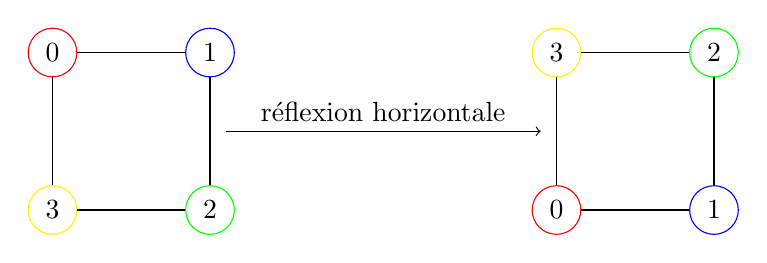
\begin{tikzpicture}
\node[draw=red,circle](A) at  (0,0) {$0$};
\node[draw=blue,circle](B) at (2,0) {$1$};
\node[draw=green,circle](C) at (2,-2) {$2$};
\node[draw=yellow,circle](D) at (0,-2) {$3$};
\draw (A) -- (B);
\draw (B) -- (C);
\draw (C) -- (D);
\draw (D) -- (A);
\draw [->] (2.2,-1) -- (6.2,-1) node [midway, above] {réflexion horizontale};
\node[draw=red,circle](A) at  (6.4,-2) {$0$};
\node[draw=blue,circle](B) at (8.4,-2) {$1$};
\node[draw=green,circle](C) at (8.4,0) {$2$};
\node[draw=yellow,circle](D) at (6.4,0) {$3$};
\draw (A) -- (B);
\draw (B) -- (C);
\draw (C) -- (D);
\draw (D) -- (A);
\end{tikzpicture}\\
\begin{Titre}
 Les sommets du carré sont identifiés par une couleur et une nombre.
\end{Titre}
\end{Figure}
\end{center}
Deux symétries quelconques peuvent être composées, c'est-à-dire appliquées l'une après l'autre.
\end{Exemple}

\begin{Remarque}
Lors de l'introduction d'un groupe $(G,*)$, on omet de mentionner la loi $*$ afin d'alléger les notations.\\
L'ensemble $G$ ne peut pas être vide car il contient au moins l'élément neutre.
\end{Remarque}
\subsection{Sous-groupes}
\begin{Definition}[Sous-Groupe]
Soit $(G, *)$ un groupe et $H$ une partie de $G$.\\
$(H, *)$ est un \defi{sous-groupe} de $(G, *)$  si $H$ est stable pour $*$ et, muni de la loi induite, est un groupe.
\end{Definition}





%\begin{Exemple}[Le Groupe \((\R^n,+)\) ]
%La loi d'addition sur $\R^n$ est définie par 
%$$ \Fonction{+}{\R^n\times\R^n}{\R^n}{(\vec{x}=(x_1,x_2,\dots,x_n),\Vect{y}=(y_1,y_2,\dots,y_n))}{\Vect{x}+\Vect{y}=(x_1+y_1, x_2+y_2, \dots, x_n+y_n)}.$$
%
%\begin{itemize}
%\item  \defi{associative} : Soit $\Vect{x}=(x_1,x_2,\dots,x_n),\Vect{y}=(y_1,y_2,\dots,y_n),\Vect{z}=(z_1,z_2,\dots,z_n)\in\R^n .$\\
% On a :
% $$\begin{aligned}
% \Vect{x}+(\Vect{y}+\Vect{z})&=(x_1,x_2,\dots,x_n)+\left((y_1,y_2,\dots,y_n)+(z_1,z_2,\dots,z_n)\right)\\
% &=(x_1,x_2,\dots,x_n)+(y_1+z_1, y_2+z_2, \dots, y_n+z_n)\\
% &=(x_1+y_1+z_1, x_2+y_2+z_2, \dots, x_n+y_n+z_n)\\
%  &=(x_1+y_1, x_2+y_2, \dots, x_n+y_n)+(z_1,z_2,\dots,z_n)\\
%  &=\left((x_1,x_2,\dots,x_n)+(y_1,y_2,\dots,y_n)\right)+(z_1,z_2,\dots,z_n)\\
%  &=(\Vect{x}+\Vect{y})+\Vect{z}
% \end{aligned}$$
% \item  \defi{commutative} : Soit $\Vect{x}=(x_1,x_2,\dots,x_n),\Vect{y}=(y_1,y_2,\dots,y_n)\in\R^n .$\\
% On a :
% $$\begin{aligned}
% \Vect{x}+\Vect{y}&=(x_1,x_2,\dots,x_n)+(y_1,y_2,\dots,y_n)\\
%  &=(x_1+y_1, x_2+y_2, \dots, x_n+y_n)\\
%  &=(y_1+x_1, y_2+x_2, \dots, y_n+x_n)\\
%  &=\Vect{y}+\Vect{x}
% \end{aligned}$$
% \item  \defi{élément neutre} : Soit $\Vect{x}=(x_1,x_2,\dots,x_n)\in\R^n$\\
% Montrons que $\Vect{0}=(0,0,\dots,0)$ est l'élément neutre\\
% On a :
% $$\begin{aligned}
% \Vect{x}+\Vect{0}&=(x_1+0,x_2+0,\dots,x_n+0)\\
%  &=(x_1, x_2, \dots, x_n)\\
%  &=\Vect{x}
% \end{aligned}$$
%  \item  \defi{symétrique} : Soit $\Vect{x}=(x_1,x_2,\dots,x_n)\in\R^n$\\
% Montrons que $-\Vect{x}=(-x_1,-x_2,\dots,-x_n)$ est l'opposé de $\Vect{x}$.\\
% On a :
% $$\begin{aligned}
% \Vect{x}+(-\Vect{x})&=(x_1,x_2,\dots,x_n)+(-x_1,-x_2,\dots,-x_n)\\
%  &=(x_1-x_1, x_2-x_2, \dots, x_n-x_n)\\
%  &=(0, 0, \dots, 0)\\
%  &=\Vect{0}
% \end{aligned}$$
%\end{itemize}
%Donc $(\R^n,+)$ est un groupe commutatif.
%\end{Exemple}




%\begin{Definition}[Corps \(\K\) : \(\R\) ou \(C\)] Dans ce cours%\samepage\footnote{%\begin{tiny}
%%Un \defi{corps} (commutatif) $(K,+,\times )$ est un ensemble muni de deux lois internes possédant les propriétés suivantes :
%%\begin{itemize}
%%\item $(K,+)$ est un groupe abélien, dont l'élément neutre est noté $0$ ;
%%\item $(K\setminus \{0\},\times )$ est également un groupe abélien, dont l'élément neutre est noté $1$ ;
%%\item $\times$ est distributive par rapport à $+$.
%%\end{itemize}
%%\impo{Remarque} Lorsque le contexte est clair, on écrit souvent $\K$ au lieu de $(\K,+,×)$.\\
%%\impo{Exemples}
%%\begin{itemize}
%%\item le corps des réels $\R$, des complexes $\C$, des rationnels $\Q$;
%%\item si $\K$ est un corps, le corps des fractions rationnelles à coefficients dans $\K$, noté $\K(X)$;
%%\item $\Q [i] = \{a+ib:(a,b)\in \Q ^2\}$;
%%\item le corps des entiers modulo un nombre premier $p$, noté $\Z/p\Z$.
%%\end{itemize}
%%}
%, un corps $\K$ désigne soit l'ensemble des nombres réels $\R$ ou soit l'ensemble des nombres complexes $\C$. 
%\end{Definition}
%\begin{Definition}[Espace vectoriel : \(\lambda\Vect{x}+\mu\Vect{y}\)]
%Soit $\K$ un corps.\\
%Un \defi{$\K$-espace vectoriel} est un triplet $(E,+,.)$ où
%$+$ est une loi de composition interne sur $E$ et
%$.$ est une loi de composition externe sur $E$,
%vérifiant les propriétés suivantes:
%\begin{enumerate}
%\item $(E, +)$ est un groupe commutatif;
%\item la loi $.$ est compatible avec la structure de groupe $(E, +)$, i.e.  
% \begin{enumerate}
%  \item $\forall(\lambda ,\mu )\in\K^2$, $\forall \Vect{x}\in E$, $(\lambda +\mu ) . \Vect{x} = (\lambda . \Vect{x}) + (\mu . \Vect{x})$;
%  \item $\forall\lambda \in\K$, $\forall(\Vect{x},\Vect{y})\in E^2$, $\lambda . (\Vect{x}+\Vect{y}) = (\lambda . \Vect{x}) + (\lambda . \Vect{y})$;
%  \item $\forall\Vect{x}\in E$, $1_\K. \Vect{x} = \Vect{x}$;
%  \item $\forall(\lambda ,\mu )\in\K^2$, $\forall\Vect{x}\in E$, $\lambda . (\mu . \Vect{x}) = (\lambda \mu ) . \Vect{x}$.
%  \end{enumerate}
%\end{enumerate}
%Un élément d'un $\K$-espace vectoriel est appelé un \defi{vecteur} et est noté dans ce cours avec une flèche  $\Vect{x}$. Un élément du corps $\K$ est un \defi{scalaire} et est noté dans ce cours à l'aide d'une lettre grecque, $\lambda$.   
%\end{Definition}
%
%
%\begin{Exemple}
%
%\begin{itemize}
%\item les n-uplets $\K^n$ muni des lois usuelles, 
%\item
%  les matrices $\mathcal{M}_{n,p}(\K)$ muni des lois usuelles,
%\item
% si $X$ est un ensemble et $E$ un $\K$-espace vectoriel, l'ensemble des fonctions $\mathcal{F}(X,E)$ muni des lois usuelles.
%\end{itemize}
%\end{Exemple}


\end{document}
